\chapter{Obsah DVD}
\label{obsahDVD}

\begin{itemize}
  \item \textbf{BarcodesLibrary/} -- C++ knihovna pro detekci a dekódování QR
  kódů
  	\begin{itemize}
  	  \item \textbf{src/} -- Zdrojové kódy knihovny
  	  \item \textbf{doc/} -- Programová dokumentace knihovny v HTML formátu
  	  \item \textbf{lib/} -- Výstupní složka pro sestavenou knihovnu
  	  \item \textbf{tests/} -- Složka obsahující zdrojové kódy pro sestavení
  	  testů kníhovny
	\end{itemize}
  \item \textbf{Doc/} -- Technická zpráva
  	\begin{itemize}
  	  \item \textbf{out/QrReader.pdf} -- Technická zpráva ve formátu PDF
	\end{itemize}
  \item \textbf{DocomoDecoderPlugin/} -- Plugin obsahující dekódér
  specifické aplikační vrstvy, který lze doinstalovat do aplikace čtečky QR
  kódů.
  	\begin{itemize}
  	  \item \textbf{src/} -- Zdrojové kódy pluginu
  	  \item \textbf{dest/DocomoDecoderPlugin.jar} -- Plugin ve formě archivu JAR,
  	  obsahující třídy zkompilované pro Dalvik VM.
	\end{itemize}
  \item \textbf{GNUMake\_OSSLib/} -- GNU Make knihovna s makry pro překlad C++
  knihovny (BarcodesLibrary)
  \item \textbf{OpenCV/} -- Sestavená OpenCV knihovna pro cílové mobilní
  architektury procesorů ARM a ARMv7a.
  \item \textbf{QRReader/} -- Aplikace čtečky QR kódu pro Android
  	\begin{itemize}
  	  \item \textbf{src/} -- Zdrojové kódy aplikace
  	  \item \textbf{doc/} -- Programová dokumentace aplikace v HTML formátu
  	  \item \textbf{dest/QRReader.apk} -- Sestavená výsledná aplikace čtečky QR
  	  kódu pro Android.
	\end{itemize}
\end{itemize}

\chapter{Ukázka výpočtu bitů korekce pro metainformace QR kódu}
\label{ukazkaVypoctuECCMetainformace}

V blocích metainformací QR kódu jsou vždy přidávány za samotné informační bity i
bity korekce chyby. Pro výpočet těchto bitů se využívá 
cyklických Bose-Chaudhuri-Hocquenghem kódů, zkráceně BCH. Redundantní bity
jsou tvořeny generujícími polynomy $G(x)$, jejichž tvar je pevně stanoven. Pro
kódování metainformace formátu QR kódu je konkrétně využito kódu BCH(15, 5)\footnote{BCH($n$, $k$) -- Zápis pro Bose-Chaudhuri-Hocquenghem kódy, kde $n$ udává, na kolika bitech bude výsledný řetězec bloku metainformace 
(včetně korekci) a $k$, pro kolik informačních bitu je korekce chyby počítána.} 
a pro kódování metainformace verze QR kódu BCH(18, 6). \cite{ISO180042006}

\bigskip \noindent Generující polynom formátu QR kódu:
\begin{equation}
G(x) = x^{10} + x^8 + x^5 + x^4 + x^2 + x + 1
\end{equation}

\noindent Generující polynom verze QR kódu:
\begin{equation}
G(x) = x^{12} + x^{11} + x^{10} + x^9 + x^8 + x^5 + x^2 + 1
\end{equation}

\bigskip \noindent Zabezpečení informačních bitů probíhá s využitím vztahu 
\begin{equation}
  \frac{f(x) x^{n-k}}{G(x)} = h(x) + \frac{r(x)}{g(x)}
\end{equation}
\noindent kde redundantní bity jsou zjištěny jako zbytek po dělení generujícím
polynomem $G(x)$. \cite{BCHCodesLiterature}

\subsubsection{Postup výpočtu redundatních bitu verze QR kódu}
\noindent -- vstupní informační bity: $000111$ (verze 7)

\begin{enumerate}
  \item Převedení binárního řetězce informačních bitů do polynomického tvaru:
	\begin{equation}
	  000111 \Rightarrow x^2 + x + 1
	\end{equation}
  \item Zvýšení mocnin polynomu v závislosti na BCH($n$, $k$) o $n - k$ pozic,
  neboli vynásobení polynomem $x^{n-k}$, zde BCH(18, 6):
	\begin{equation}
	  x^2 + x + 1 \Rightarrow x^{14} + x^{13} + x^{12}
	\end{equation}
  \item Vydělení vzniklého polynomu generujícím polynomem:
	\begin{equation}
	  \frac{x^{14} + x^{13} + x^{12}}{G(X)} =  x^2 + \frac{x^{11} + x^{10} + x^7 +
	  x^4 +x^2}{x^{12} + x^{11} + x^{10} + x^9 + x^8 + x^5 + x^2 + 1}
	\end{equation}
  \item Převod zbytku po dělení na binární řetězec (redundatních bitů):
	\begin{equation}
      x^{11} + x^{10} + x^7 + x^4 +x^2 \Rightarrow 110010010100
	\end{equation}
  \item Konkatenace informačních bitů a jejich redundatních bitů korekce chyby:
	\begin{equation}
      000111 + 110010010100 \Rightarrow 000111110010010100
	\end{equation}
  \item Aplikace XOR masky $101010000010010$, jedná li se o kódování
  metainforamce formátu QR kódu, k zamezení vzniku binárního řetězce s
  nulovými bity ve všech pozicích.
\end{enumerate}

\chapter{Algoritmus pro hledání rohů polygonu}
\label{algoritmusHledaniRohu}

Algoritmus hledání rohů polynomu byl navržen pro hledání čtyř bodů (rohů)
poziční značky, která byla definovaná množinou bodů, jež ohraničovaly danou
značku. Obecně lze ovšem algoritmus použít pro jakýkoliv polynom, princip jeho
činnosti můžeme vidět na obrázku \ref{prilohaHledaniRohuObr}.

\begin{figure}[H]
  \begin{center}
    \scalebox{0.25}{
      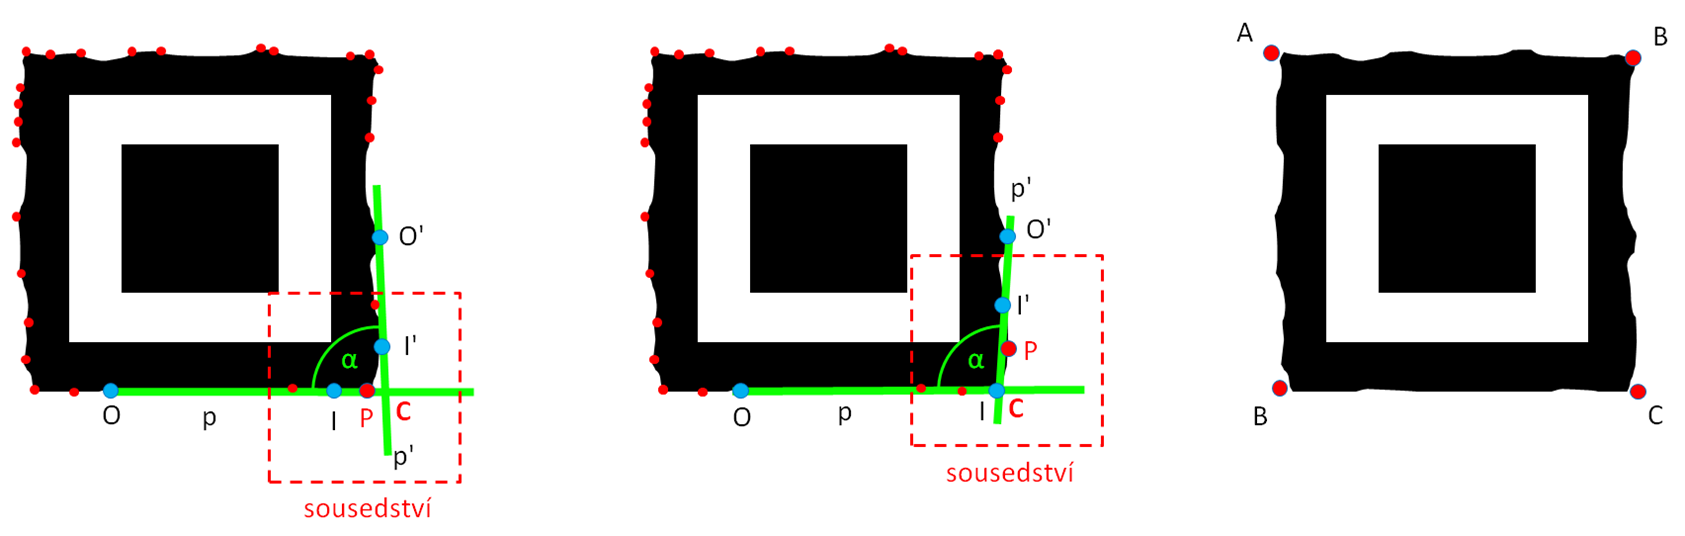
\includegraphics{fig/SearchCornersOfPolygonAlgorithm.PNG}
    }
    \caption{Zobrazení dvou kroků algoritmu a výsledku hledání rohů polynomu}
    \label{prilohaHledaniRohuObr}
  \end{center}
\end{figure}

\noindent Vstupními parametry algoritmu jsou:
\begin{itemize}
  \item Velikost sousedství v pixelech $V$
  \item Interval povolených úhlů $R$, jež mohou svírat přímky $p$ a $p'$, aby
  jejich průsečík byl uznán jako roh polygonu. 
\end{itemize}

\subsubsection{Slovní popis algoritmu}
\begin{enumerate}
  \item Pokud množina bodů kontur obsahuje méně než tři body, skonči.
  \item Pro každý bod kontury vytvoř strukturu, která obsahuje body $I$, $O$,
  $I'$ a $O'$.
	\begin{enumerate}
	  \item Obsahuje-li sousedství právě zpracovávaného bodu ve směru hodinových 
	  ručiček alespoň jeden bod, ulož do $I$ právě ten nejbližší v daném směru, 
	  jinak ulož do $I$ právě zpracovávaný bod. Totéž proveď i ve směru proti 
	  směru hodinových ručiček a nastav bod $I'$.
	  \item Existuje-li mimo sousedství právě zpracovávaného bodu alespoň jeden
	  bod, ulož do $O$ nejbližší bod mimo sousedství ve směru hodinových ručiček.
	  Neexistuje-li mimo sousedství právě zpracovávaného bodu žádný bod a v $I$
	  není nastaven právě zpracovávaný bod, ulož do $O$ právě zpracovávaný bod.
	  Neexistuje-li mimo sousedství právě zpracovávaného bodu žádný bod a v $I$
	  je nastaven právě zpracovávaný bod, ulož do $O$ nejbližší bod ve směru
	  hodinových ručiček od právě zpracovávaného bodu. Totéž proveď i ve směru
	  proti směru hodinových ručiček a nastav bod $O'$ s ohledem na $I'$.
	\end{enumerate}
  \item Projdi všechny vytvořené struktury a sestroj z bodů $I$ a $O$ přímku $p$
  a z bodů $I'$ a $O'$ přímku $p'$. Zjisti úhel $\alpha$, jež svírají obě dvě
  přímky a v případě, že $\alpha \in E$, vlož průsečík tšchto přímek do seznamu
  získaných rohů $S$.
  \item Projdi všechny získané rohy $S$ a ověř, zda se v sousedství rohů
  nenachází jiný z nalezených rohů. Pokud je nalezen v sousedství nějakého rohu jiný roh,
  odstraň oba dva rohy a vlož do seznamu rohů nový roh daný aritmetickým
  průměrem souřadnic obou rohů a opakuj krok 4, dokud sousedství každého rohu
  není prázdné. 
\end{enumerate}

%\chapter{Manual}
%\chapter{Konfigrační soubor}
%\chapter{RelaxNG Schéma konfiguračního soboru}
%\chapter{Plakat}

